\documentclass[10pt,twocolumn,letterpaper]{article}

% CVPR author-kit style (https://github.com/cvpr-org/author-kit): letter paper,
% Times 10pt, 6.875in x 8.875in text block, 0.3125in column gap. It already loads
% graphicx, amsmath, amssymb, booktabs, xcolor, natbib and enumitem.
% Option `pagenumbers' keeps page numbers (CVPR final mode hides them).
\usepackage[pagenumbers]{cvpr}

\usepackage{multirow}
\usepackage{placeins}
\usepackage[breaklinks=true,colorlinks,bookmarks=false,linkcolor=blue!50!black,citecolor=blue!50!black,urlcolor=blue!50!black]{hyperref}
\usepackage[capitalize]{cleveref}

\graphicspath{{figures/}{../figures/}}

% Outline notes; set \showoutline to false to hide them in the final version.
\newif\ifshowoutline \showoutlinetrue
\newcommand{\outline}[1]{\ifshowoutline{\color{gray}\small\itshape [Outline] #1\par}\fi}

% Expected (not yet measured) results: shown in blue; replace with measured text, then
% delete the macro. Set \showexpected to false to hide them.
\newif\ifshowexpected \showexpectedtrue
\newcommand{\expect}[1]{\ifshowexpected{\color{blue!60!black}#1}\fi}
% Placeholder for a result figure that is not produced yet: \figph{width}{height}{text}
\newcommand{\figph}[3]{\fbox{\parbox[c][#2][c]{\dimexpr#1-2\fboxsep-2\fboxrule\relax}{\centering\small\color{gray}#3}}}

\title{How Much Does Time Matter?\\
A Comparative Study of Aggregation, Temporal Patterns, Dynamics\\and Community Evolution in Real-World Temporal Networks}
% CVPR-style author block for authors sharing one affiliation and one email domain:
% names on one line, shared affiliation, then \{id1, id2, ...\}@domain.
\newcommand{\sharedaffiliation}{Faculty of Science, National University of Singapore}
\newcommand{\emailids}{}
\newcommand{\emaildomain}{u.nus.edu}
\author{%
  Author One, Author Two, Author Three, Author Four, Author Five\\
  \sharedaffiliation\\
  {\small\texttt{\{\emailids\}@\emaildomain}}
}

\begin{document}
\maketitle

\begin{abstract}
Real networks are made of interactions that happen at specific times, yet they are
routinely analysed as static aggregated graphs. We ask how much this discards. We
organise the temporal-network literature around four questions---representation,
activity patterns, structural evolution and function---distil seven testable
hypotheses (H1--H7), and define a common pipeline of window analysis,
randomized reference models and dynamic-community tracking on three networks of
different type and time scale: face-to-face contacts in a primary school, online
messaging among students, and a computer-science citation network. The planned cross-network comparison
uses normalised \emph{time effects} rather than raw metrics.
The completed citation-network study contains 19,150 papers and 73,269
strictly older-target citations. It supports sublinear degree preference and
age-dependent citation choice, with a densification exponent of 1.343, but no
detected shrinkage of the sampled effective diameter. A three-parameter citation
model fits selected histories well without an established MAE advantage over
linear extrapolation. Contact and messaging experiments remain pending, so a
cross-network ranking of temporal sensitivity is not yet inferred.
\end{abstract}

%=====================================================================
\section{Introduction}
\label{sec:intro}
Real networks evolve: nodes and links appear and disappear, and interactions take
place at specific moments---a conversation lasts a minute, a message is sent at a
given second, a paper cites earlier work in a given year. Classical network analysis
nevertheless collapses all of this into one static graph in which two nodes are either
linked or not. Such aggregation is convenient, but it discards when links are active,
how often they recur, in which order they occur and how the network changes. Unlike
for static graphs, connectedness is not transitive in time, so a temporal network cannot
be reduced to a simple graph without loss \citep{holme2015modern}. The
temporal-network literature \citep{holme2012temporal,holme2015modern,masuda2016guide}
has shown that each of these ingredients can change the conclusions drawn about
structure, communities, and processes such as epidemics.

Most of this evidence, however, comes from a single dataset or a single method. It
is therefore hard to tell \emph{how much} time matters in general, and for which kinds
of systems. We address two research questions.
\textbf{RQ1:} how does temporal information change our understanding of the structure
and function of real networks, and how does this effect differ across network types?
\textbf{RQ2:} which hypotheses from the temporal-network literature (H1--H7,
\cref{tab:hypotheses}) hold in which systems?

\paragraph{Approach.}
The report is organised around four questions that recur in every section
(\cref{fig:framework}): (I) \emph{representation}---what is lost by aggregation and
by the choice of time window? (II) \emph{activity patterns}---are interactions bursty,
repeated and persistent? (III) \emph{structural evolution}---how do networks grow,
age and reorganise? (IV) \emph{function}---does time ordering change reachability,
centrality and spreading? Each question is turned into a literature hypothesis, a
metric and a randomized reference model \citep{gauvin2022randomized}, and applied to
three networks that differ in edge meaning, generating mechanism and time scale
(seconds, seconds, years): face-to-face contacts, online messages and citations.
Because raw metrics are not comparable across such systems, datasets are compared via
\emph{normalised time effects} (\cref{sec:time-effect}). We do not propose new
models; the contribution lies in the common framework and the comparison.

\begin{figure*}[t]
\centering
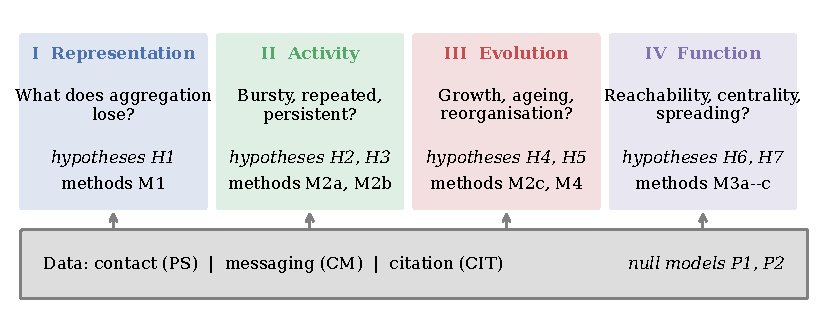
\includegraphics[width=\textwidth]{fig_framework.pdf}
\caption{Structure of the study. Four questions (Parts I--IV) map to seven
hypotheses and four method groups; the same order is used in Related Work, Methods,
Results and Discussion. All analyses use the same three datasets and the same
randomized reference models.}
\label{fig:framework}
\end{figure*}

\paragraph{Contributions.}
(1) A question-driven synthesis of how network scientists study temporal networks;
(2) a common, reproducible pipeline that applies it to three types of real data;
(3) a cross-network verdict on H1--H7, stating where time information is essential and
where a static view suffices.

\paragraph{Roadmap.}
\Cref{sec:related} reviews related work, \cref{sec:data} describes the data,
\cref{sec:methods} the methods, \cref{sec:results} the results,
\cref{sec:discussion} discusses them and \cref{sec:conclusion} concludes.

%=====================================================================
\section{Related Work}
\label{sec:related}
We organise the literature by question rather than paper by paper; the subsections
follow Parts I--IV of the Introduction. General frameworks and reviews are given by
\citet{holme2012temporal,holme2015modern} and the book of \citet{masuda2016guide}.
A central point of these reviews is that the basic unit is a \emph{contact}
(two nodes and a time), and that connectedness is no longer transitive: if $a$ meets
$b$ and later $b$ meets $c$, a path from $a$ to $c$ exists, but not the other way
round. Hence a temporal network cannot be turned into a simple graph without losing
information or changing what a node means, and many static-network methods need
non-trivial generalisations \citep{holme2015modern}.

\subsection{Representing time: aggregation, snapshots and windows}
\label{sec:rw-representation}
Temporal networks can be stored as contact sequences, interval graphs or sequences of
snapshots \citep{holme2012temporal}. Lossy representations such as weighted aggregates or reachability graphs reduce the
data to a static object; lossless ones keep all contacts \citep{holme2015modern}.
Each choice involves a trade-off: snapshots
make static tools applicable but require a window length, whereas the full event
sequence keeps all information. The effect of this choice has been quantified for
communication data: window size and placement change the structure of the aggregated
network \citep{krings2012effects}, and coarser temporal resolution distorts
properties of the time-varying network in a way that depends on the system
\citep{ribeiro2013quantifying}. This motivates \textbf{H1}: aggregation and window
choice change structural conclusions.

\subsection{Temporal activity patterns}
\label{sec:rw-activity}
Human activity is bursty: inter-event times are heavy-tailed rather than exponential
\citep{barabasi2005origin}, and consecutive intervals are correlated, which
\citet{goh2008burstiness} capture with a burstiness coefficient and a memory
coefficient. Social ties are also repeated and persistent over long periods
\citep{saramaki2014persistence}, while the set of active links turns over. Temporal motifs
\citep{kovanen2011temporal,paranjape2017motifs} and activity-driven models
\citep{perra2012activity} describe and generate such patterns. This gives
\textbf{H2} (activity is bursty and has memory) and \textbf{H3} (ties are repeated and
persistent while the network turns over).

\subsection{Structural evolution: growth, ageing and communities}
\label{sec:rw-evolution}
Growth is classically explained by preferential attachment
\citep{barabasi1999emergence}, whose strength can be measured directly from
growth data \citep{jeong2003measuring,newman2001clustering}. Real systems usually
show ageing, where old nodes attract fewer new links
\citep{dorogovtsev2000aging}, and in citations this is captured by a relevance
decay \citep{wang2013quantifying}. Growing networks also densify, with the number of
edges growing superlinearly in the number of nodes
\citep{leskovec2005graphs,leskovec2007graph}; node and link deletion alter these
laws \citep{moore2006exact}. This gives \textbf{H4}: growth follows preferential
attachment with ageing, and networks densify.

At the mesoscale, multilayer modularity couples partitions across time
\citep{mucha2010community}, communities can be tracked across snapshots through
matching \citep{greene2010tracking} and change can be mapped between partitions
\citep{rosvall2010mapping}; \citet{rossetti2018community} survey the field. Per-snapshot
partitions are typically obtained with Louvain \citep{blondel2008fast} or Leiden
\citep{traag2019louvain}. This gives \textbf{H5}: communities reorganise over time and
a static partition hides this.

\subsection{Time and network function}
\label{sec:rw-function}
Because interactions occur in sequence, only time-respecting paths can carry
information: reachability in contact sequences is much lower than in the aggregated
graph \citep{holme2005network}, and path lengths and centrality change accordingly
\citep{pan2011path,kim2012temporal}. Burstiness and temporal correlations further
slow down spreading even when the static topology is unchanged
\citep{karsai2011small}. These results give \textbf{H6} (time ordering restricts
reachability and changes centrality rankings) and \textbf{H7} (burstiness and
temporal correlations slow down spreading).

\subsection{Randomized reference models}
\label{sec:rw-null}
Randomization is more versatile for temporal than for static networks, where it is
essentially limited to degree-preserving link shuffling, because one can switch off
individual kinds of correlation \citep{holme2015modern}. Randomized reference models act as hypothesis tests: each one preserves some
properties of the data and destroys others, so differences between data and model
reveal which feature matters \citep{gauvin2022randomized}. We use them in Parts
II--IV (\cref{sec:null}).

\paragraph{Time scales and network types.}
Temporal networks are usually defined as systems whose evolution is not much slower
than the processes running on them, and a single system contains many time scales
(seconds, hours, days) \citep{holme2015modern}. Contact and communication data are
event sequences with such a hierarchy, whereas citation networks are acyclic by
construction and all out-links of a paper appear at one instant
\citep{holme2015modern}. This is why we expect, and test, different sensitivity to time
across network types.

\paragraph{Gap.}
Most studies examine one dataset or one method. Few compare, within a single
framework, how sensitive different \emph{types} of networks are to temporal
information. The hypotheses distilled above (\cref{tab:hypotheses}) allow such a
comparison.

%=====================================================================
\section{Data}
\label{sec:data}
We use one network per type, chosen to differ in edge meaning, generating mechanism and time scale (seconds, seconds, years); data cards are in \cref{tab:data} and activity time series in \cref{fig:activity}.

\begin{table}[t]
\centering
\small
\setlength{\tabcolsep}{3pt}
\begin{tabular}{@{}llrrll@{}}
\toprule
Type & Dataset & $N$ & Events & Span & Res. \\
\midrule
Contact & Primary school (PS) & 242 & 125\,773 & 2 d & 20 s \\
Comm. & CollegeMsg (CM) & 1\,899 & 59\,835 & 193 d & 1 s \\
Citation & DBLP--DB (CIT) & 19\,150 & 73\,269 & 50 yr & 1 yr \\
\bottomrule
\end{tabular}
\caption{Data cards. $N$: nodes; Res.: temporal resolution. CIT spans publication years 1970--2020, with primary analysis in 1990--2020. PS: undirected, class labels, CC BY-NC-SA;
CM: directed, no labels; CIT: directed, acyclic.}
\label{tab:data}
\end{table}

\paragraph{Face-to-face contact.}
The primary-school data \citep{stehle2011high,gemmetto2014mitigation} were collected by
the SocioPatterns collaboration with wearable proximity sensors over two school days.
A contact is recorded when two people are face to face within about 1.5\,m for at
least 20\,s. Each individual carries a class label, which we use as ground truth for
communities. The data are released under CC BY-NC-SA.

\paragraph{Online communication.}
CollegeMsg \citep{panzarasa2009patterns} contains time-stamped private messages
between 1\,899 users of an online student community over 193 days at 1\,s
resolution. Edges are directed, and there are no node labels.

\paragraph{Scientific publications.}
% Owner: B (measured CIT data card).
We use AMiner DBLP-Citation V14 \citep{tang2008arnetminer}, selected by a fixed
set of database venue families and their declared name variants. Streaming
5,259,858 records yields 19,150 publications from 1970--2020 and 73,269 distinct
citations to strictly older selected papers. These are within-subgraph citations,
not global citation counts; 6,709 nodes are isolates. We save 5,486 same-year
references separately, exclude 6,390 later-year references and 494 self-loops,
and remove 37,440 repeated reference entries. The graph is acyclic under the
strict year rule. AMiner specifies research use; no additional open-data licence
is inferred. The recent fall in observed references despite growing paper counts
motivates a cutoff-2015 sensitivity check and cautions about coverage and censoring.

\paragraph{Preprocessing.}
All data are converted to a common event format $(u,v,t)$ with integer time stamps
(seconds or years) plus a table of node labels. Self-loops and exact duplicate
events are removed, and the first and last partial windows are trimmed. Each source
has known limits: citation data have year-level resolution, the contact data cover only
two days, and the sensors sample only participants who wear them. The three datasets
differ in edge meaning (proximity, message, citation), directedness and time scale
by design, so that agreement across them is not an artefact of one data type.

\begin{figure*}[t]
\centering
\figph{0.46\textwidth}{1.7cm}{PS: events per hour\\Pending A's measured series}\hfill
\figph{0.46\textwidth}{1.7cm}{CM: events per hour\\Pending A's measured series}
\par\medskip
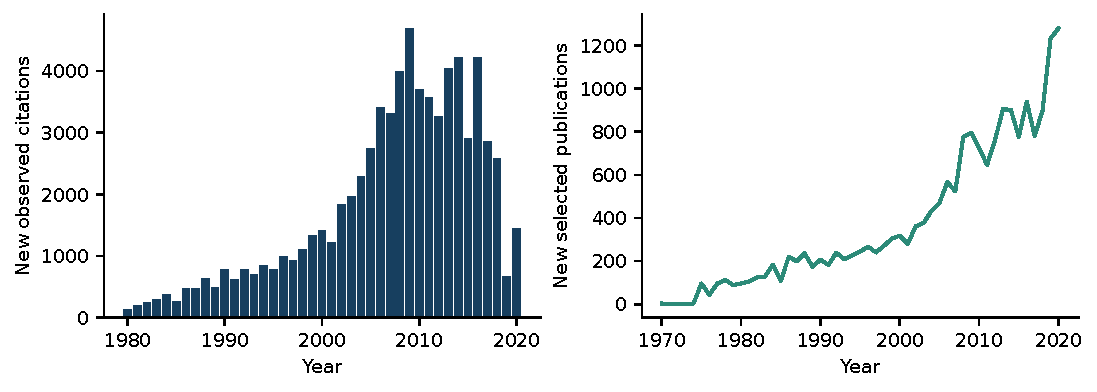
\includegraphics[width=.95\textwidth]{b_activity.pdf}
\caption{Activity overview. The lower panels are measured CIT annual citations
and selected publications; upper panels reserve the pending PS/CM series.
CIT's late reference decline alongside rising publication counts motivates
coverage and observation-cutoff checks.}
\label{fig:activity}
\end{figure*}

%=====================================================================
\section{Methods}
\label{sec:methods}
Every analysis follows the same template: hypothesis from the literature $\to$ metric
$\to$ randomized reference model. \Cref{tab:hypotheses} lists the seven hypotheses,
the methods (M1--M4) that test them and the datasets where each method is meaningful
(19 method--dataset pairs). The empty cells are deliberate: CIT is a year-resolution
DAG without fine-grained events (no M2a, M2b, M3) and without community
reorganisation (no M4), while PS and CM have no growth process (no M2c).

\begin{table*}[t]
\centering
\small
\setlength{\tabcolsep}{4pt}
\begin{tabular}{@{}cl p{6.2cm} l l l ccc@{}}
\toprule
Part & ID & Hypothesis & Source & Method & Null & PS & CM & CIT \\
\midrule
I   & H1 & Aggregation and window choice change structural conclusions
           & \citep{krings2012effects,ribeiro2013quantifying} & M1 & -- & \checkmark & \checkmark & \checkmark \\
\midrule
II  & H2 & Activity is bursty and has memory
           & \citep{goh2008burstiness} & M2a & P1 & \checkmark & \checkmark & \\
    & H3 & Ties are repeated and persistent; the network turns over
           & \citep{saramaki2014persistence} & M2b & P1 & \checkmark & \checkmark & \\
\midrule
III & H4 & Growth follows preferential attachment with ageing; networks densify
           & \citep{jeong2003measuring,wang2013quantifying,leskovec2005graphs} & M2c-1--4 & P3 & & & \checkmark \\
    & H5 & Communities reorganise over time; the static partition hides this
           & \citep{greene2010tracking,mucha2010community} & M4 & P1 & \checkmark & \checkmark & \\
\midrule
IV  & H6 & Time ordering restricts reachability and changes centrality rankings
           & \citep{holme2005network,pan2011path,kim2012temporal} & M3a, M3b & P1, P2 & \checkmark & \checkmark & \\
    & H7 & Burstiness and temporal correlations slow down spreading
           & \citep{karsai2011small} & M3c & P1, P2 & \checkmark & \checkmark & \\
\bottomrule
\end{tabular}
\caption{Hypotheses tested in this work, with methods, null models
(\cref{sec:null}) and applicable datasets.}
\label{tab:hypotheses}
\end{table*}

\subsection{Notation}
\label{sec:notation}
Let $\mathcal{E}=\{(u,v,t)\}$ be the event sequence. The static aggregate $G$
contains a link $(u,v)$ if at least one event occurs between $u$ and $v$. A
snapshot $G_{\Delta t}(k)$ contains the events in $[k\Delta t,(k+1)\Delta t)$, and the
cumulative network $G(\le t)$ contains all events up to $t$.

\subsection{Aggregation and time windows (M1)}
\label{sec:m-aggregation}
For each window length $\Delta t$ on a grid (PS: 5\,min to 1\,day; CM: 1\,h to 1\,month)
we compute density, mean degree, clustering coefficient and giant-component size of the
snapshots and of the aggregate. For CIT, yearly and cumulative networks are compared.
\emph{Window sensitivity} is the relative change of a metric across the grid.
Rankings are handled separately in M3b. \Cref{fig:aggschem} shows why aggregation can
mislead: a path present in the static graph may not be traversable in time.

\begin{figure*}[t]
\centering
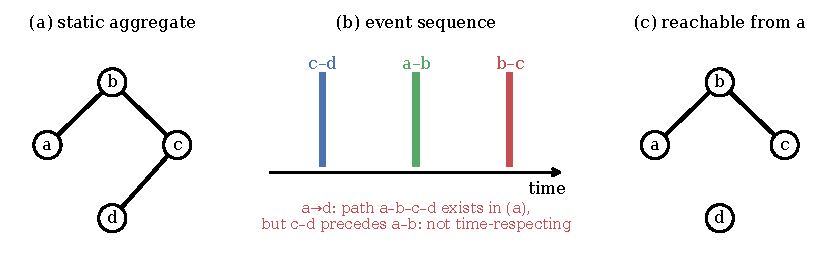
\includegraphics[width=0.7\linewidth]{fig_aggregation_schematic.pdf}
\caption{Aggregation adds paths that do not exist in time. In (a) $a$ appears to
reach $d$; in (b) the link $c$--$d$ is active before $a$--$b$, so in (c) only $b$ and
$c$ are reachable from $a$.}
\label{fig:aggschem}
\end{figure*}

\subsection{Activity patterns (M2a, M2b)}
\label{sec:m-activity}
\textbf{M2a} measures the inter-event time distribution of each node pair and of each
node, fitted with a heavy-tailed model, together with burstiness
$B=(\sigma-\mu)/(\sigma+\mu)$ and memory $M$, the correlation of consecutive
intervals \citep{goh2008burstiness}. \textbf{M2b} measures the edge repetition rate,
tie lifetime and the Jaccard similarity of consecutive snapshots, which quantifies
the turnover of nodes and links.

\subsection{Structural evolution (M2c, M4)}
\label{sec:m-evolution}
% Owner: B (expanded M2c-1 through M2c-4 and P3).
% Owner: B. Measured-result-independent methods, PLAN v3.1.
\paragraph{Citation data and time resolution.}
We stream AMiner DBLP-Citation V14 \citep{tang2008arnetminer} and retain an induced subgraph of database
venues selected by a fixed whitelist (SIGMOD, VLDB/PVLDB, ICDE, PODS, EDBT,
ICDT, TODS, VLDB Journal, Data \& Knowledge Engineering, and Information Systems).
All selected papers published in 1960--2020 are retained, including isolates.
A distinct citation $u\to v$ occurs in the publication year of $u$.
The primary analysis requires $y_v<y_u$; same-year citations are saved for
structural sensitivity analysis because their order cannot be resolved.
We exclude self-citations to the same paper, duplicate edges and future references.
Author self-citations are not removed. Counts refer to citations within the
selected venues, rather than global citation impact. The primary analysis years
are 1990--2020, initialized using the available earlier history.

\paragraph{M1: annual and cumulative citation structure.}
Annual and cumulative networks use the same node denominator: all selected
papers already published by year $t$. Directed density is $E/[N(N-1)]$ and
mean total degree is $2E/N$. Clustering, component counts and largest-component
fractions use the weak undirected projection, including isolates.
Trailing windows of 1, 2, 5 and 10 years provide a window-sensitivity check;
sensitivity is $(\max-\min)/\mathrm{mean}$ over the grid at each endpoint,
then averaged over endpoints.

\paragraph{M2c-1: preferential attachment.}
Following the degree-class approach of \citet{jeong2003measuring}, we freeze
in-degree at the start of each citing year and count eligible nodes $n_{tk}$ and
new citations $h_{tk}$ in each prior-degree class $k$.
We estimate $\alpha$ by conditional likelihood with probabilities proportional
to $n_{tk}(k+1)^\alpha$, conditioning on the total number of citations in each year.
The offset admits citations to previously uncited papers; offsets 0.5 and 2
provide sensitivity checks. Confidence intervals use 400 resamples of citing-year
blocks. These are descriptive uncertainty intervals; neither positive $\alpha$
nor its departure from an age-only null identifies a causal mechanism.

\paragraph{M2c-2: ageing.}
For ages 1--60, the target probability in citing year $t$ is proportional to
$n_{ta}f(a)$, where $n_{ta}$ counts available papers of age $a$.
A conditional target likelihood compares discrete-grid lognormal, exponential,
power-law and uniform kernels using AIC on identical observations and support.
We repeat the comparison by publication cohort (1970--1989, 1990--1999,
2000--2009), accounting for each cohort's actual exposure.
This estimates marginal ageing; degree, fitness and venue coverage can also
influence this curve.

\paragraph{M2c-3: densification and diameter.}
We fit $\log E(t)=a\log N(t)+b$ over 1990--2020 and repeat over split periods and
an earlier observation cutoff. Year-resampling intervals are descriptive because
cumulative observations are dependent.
Effective diameter is the 90th percentile of weak shortest-path distances
within the largest connected component, using 128 uniformly sampled source nodes
per year. Sensitivity checks use 64 and 256 sources. We save the component size
and number of sources with every estimate \citep{leskovec2005graphs}.

\paragraph{M2c-4: citation dynamics and prediction.}
We fit the Wang--Song--Barab\'asi curve \citep{wang2013quantifying},
\begin{equation}
 c(t)=m\left[\exp\!\left\{\lambda\Phi\left(\frac{\log t-\mu}{\sigma}\right)\right\}-1\right],
\end{equation}
where $m$ is fixed to the mean observed within-subgraph reference count of papers
published through 1989. Bounded multistart least squares minimizes squared
$\log(1+c)$ errors; parameter bounds and boundary flags are preserved.
For descriptive full-history fits we randomly select at most 500 papers born in
1990--2005 with at least 10 citations by age 15 and fit years 1--15. The resulting
collapse is in-sample evidence only.
For prediction, selection uses only the first five years: at least five observed
citations by age five, followed by a fixed random sample of at most 500 papers.
Using only years 1--5, we compare WSB against no-ageing PA,
$c(t)=m[\exp(rt)-1]$, and linear extrapolation, $c(5)t/5$.
All models predict the same papers at age 15 and at the observed endpoint in 2020;
these are censored observed totals, not unobserved lifetime citations.
We report MAE, median absolute error, RMSLE, paired bootstrap differences
(1000 resamples) and an interior-fit sensitivity check. Boundary fits remain in
the primary evaluation so that difficult cases are not silently discarded.

\paragraph{P3: citation-target randomization.}
Twenty realizations per model preserve each paper's publication year and exact
number of distinct observed references, with no replacement and strictly older
targets. P3a selects eligible targets uniformly. P3b weights targets by a nonparametric age kernel fitted by conditional
target likelihood, accounting for each citing year's available age distribution,
and removes degree preference.
Its age weights are calibrated from the data, so agreement on ageing is not an
independent confirmation. We report null means and sample standard deviations;
empirical tail probabilities have minimum resolution $1/21$.
Both models fix $N(t)$ and $E(t)$ and hence exactly preserve the densification
exponent. They can test diameter and target preference, but cannot supply a
significance test for densification itself.

\paragraph{Reproducibility.}
All significant CPU workloads run on Vanda compute nodes through PBS without GPU
allocation. Fixed seeds, input/source checksums, environment lock file, filtering
counts, individual forecasts and every randomized edge list are saved.
Robustness checks cover time splits, cutoff 2015, degree offsets, same-year edges,
core database venues, diameter sampling, and 10 versus 20 null realizations.


% Owner: E
% Owner: E. M4 (H5), input from methods.tex.
\textbf{M4} cuts the event sequence into consecutive windows of width $\Delta t$ and
aggregates each into a weighted undirected snapshot (weight = number of events). Windows
with very few events are dropped (fewer than 100 for PS, which removes nights; fewer
than 50 for CM), and only nodes active in a window belong to its snapshot. The main
settings are $\Delta t=15$\,min for PS and 7\,days for CM. Every snapshot and the
static aggregate are partitioned with Leiden \citep{traag2019louvain} maximising
modularity with resolution $\gamma$ \citep{reichardt2006statistical}. A multislice
partition \citep{mucha2010community} with interslice coupling $\omega=1$ gives labels
that are consistent across windows; we use it only for tracking, because the coupling
itself pulls consecutive partitions together.

Partitions are compared with NMI \citep{danon2005comparing}, always on the nodes the two
partitions share. For each window we record the NMI with the previous window (only for
back-to-back windows, not across a night), with the static partition, and for PS with
the classes (teachers excluded). As a noise floor, every window is partitioned a second
time with another random seed. All measures are recomputed on 20 P1 samples: P1 keeps
the static graph, and hence the static partition, and the number of events per window,
so H5 predicts that real snapshots agree less with each other and with the static
partition than P1 snapshots do. We repeat the analysis for $\gamma\in\{0.5,1,2\}$ and
$\Delta t\in\{5,15,60\}$\,min (PS) or $\{1,7,30\}$\,days (CM).


\subsection{Paths, centrality and spreading (M3)}
\label{sec:m-function}
\textbf{M3a} computes earliest-arrival time-respecting paths and the temporal reachability
ratio $R$ (fraction of node pairs connected by a time-respecting path, relative to the
static aggregate). \textbf{M3c} runs an event-driven SIR process on the event sequence with
at least 100 random seeds; SI with certain transmission is equivalent to M3a, so only SIR
is run.

% Owner: E
% Owner: E. M3b (H6), input from methods.tex.
\textbf{M3b} compares static and temporal closeness. Static closeness is harmonic
closeness \citep{marchiori2000harmony}, $C^{\mathrm{s}}(i)=\sum_{j\neq i}1/d(i,j)$, on
the aggregate (outgoing distances for CM), with hop distance (unweighted) or distance
$1/w_{ij}$ (weighted). Temporal closeness \citep{pan2011path,kim2012temporal} uses the
same time-respecting paths as M3a: from a start time $t_0$, an event $(u,v,t)$ can be
used only if $u$ was reached strictly before $t$, and $v$ is then reached at $t$, so no
path takes two hops within one timestamp. With $a_{t_0}(i\to j)$ the earliest arrival
time,
\begin{equation}
  C^{\mathrm{t}}(i)=\frac{1}{|\mathcal{T}|}\sum_{t_0\in\mathcal{T}}\frac{1}{N-1}
  \sum_{j\neq i}\frac{1}{a_{t_0}(i\to j)-t_0},
\end{equation}
where unreachable nodes contribute zero. $\mathcal{T}$ holds every full hour from
09:00 to 16:00 on both PS days (16 start times) and 20 evenly spaced times over the
first 90\% of the CM period. Agreement is measured by Kendall's $\tau_b$ and the overlap
of the top 10\% nodes. P1 leaves the static graph and so $C^{\mathrm{s}}$ unchanged;
recomputing $C^{\mathrm{t}}$ on 20 P1 samples therefore isolates the effect of timing.


\subsection{Randomized reference models}
\label{sec:null}
No single temporal counterpart of the configuration model exists, so one switches off
selected correlations with different models and compares the outcomes
\citep{holme2012temporal,gauvin2022randomized}. For PS and CM we use two complementary models, which
correspond to \emph{randomly permuted times} (RP) and \emph{randomized edges} (RE) in the
naming of \citet{holme2012temporal}. \textbf{P1} (RP) permutes timestamps among events:
it keeps the static graph and the number of contacts of every pair, and destroys
burstiness and temporal correlations. \textbf{P2} (RE) rewires the static graph in a
degree-preserving way while each pair's contact sequence moves with its link: it
destroys the wiring diagram but keeps per-link burstiness and the overall event rate
(\cref{fig:nullmodels}). Comparing the two separates the effect of time from that of
structure. Combined models (RE+RP) and fully random times (RT) are possible extensions. Each is run with at least
20 realisations and reported as mean $\pm$ standard deviation.

\begin{figure*}[t]
\centering
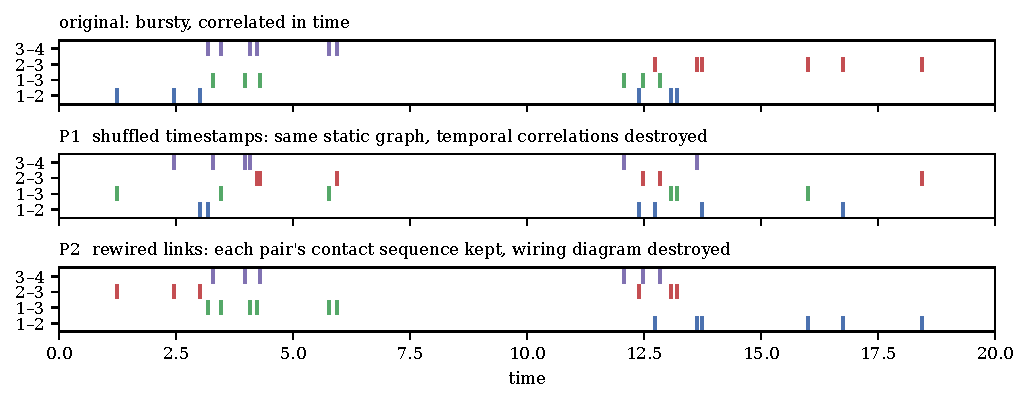
\includegraphics[width=\linewidth]{fig_nullmodels.pdf}
\caption{Toy illustration of the randomized reference models. Rows are node pairs,
ticks are events. P1 permutes the timestamps, P2 permutes which pair each event
belongs to.}
\label{fig:nullmodels}
\end{figure*}

\subsection{Measuring the effect of time}
\label{sec:time-effect}
Raw metrics cannot be compared across a contact network, a message network and a
citation network, so we define one normalised measure per hypothesis:
H1 window sensitivity (relative change of a metric over the $\Delta t$ grid);
H2 $B_{\mathrm{real}}-B_{\mathrm{null}}$;
H3 mean consecutive-snapshot Jaccard similarity;
H4 exponents $\alpha$ and $a$;
H5 mean consecutive-snapshot NMI and dynamic-vs-static NMI;
H6 reachability ratio $R$ and Kendall $\tau$(static, temporal);
H7 slowdown $T_{\mathrm{real}}/T_{\mathrm{null}}$, where $T$ is the time to the epidemic peak.

\subsection{Implementation}
All code is in Python. We use NetworkX for static graph analysis and leidenalg
\citep{traag2019louvain} for per-snapshot and multislice partitions; time-respecting
paths are computed by our own earliest-arrival code. Null models, the attachment-kernel
% E: Raphtory and tnetwork were planned but not used (M3b, M4); D to confirm for M3a.
estimator and the SIR process are custom code, unit-tested on hand-built examples
whose answers are known (reachability, SIR, preserved quantities of P1 and P2). Random
seeds are fixed and every figure is generated by one script.

%=====================================================================
\section{Results}
\label{sec:results}
The results follow the four parts of \cref{sec:methods}. Each subsection presents
the applicable datasets and their available evidence;
\cref{sec:r-cross} collects the verdicts. The CIT results below are measured outputs of all five B experiments, including
40 citation-target null graphs. Blue text elsewhere denotes untested expectations
for PS/CM, and grey boxes denote their pending figures. These draft expectations
are not evidence in the measured summary.
% One file per part; owners (PLAN.md section 5) are marked inside each file.
\subsection{Aggregation and time windows}
\label{sec:r-aggregation}

% Owner: A
\paragraph{Contact and messaging networks (PS, CM).}
\outline{Which conclusions are stable under window choice, and over which
$\Delta t$ range?}
\expect{[Expected] Density and clustering of the snapshots rise quickly with
$\Delta t$ and approach the aggregate only for windows comparable to the whole
observation period. The giant component of short-window snapshots is small, and
percolates at a window that is much shorter for CM than for PS because PS has a
daily rhythm (lessons, breaks). Conclusions about ``the'' clustering or density of
the network therefore depend strongly on $\Delta t$.}

\begin{figure*}[t]
\centering
\figph{0.32\textwidth}{3.6cm}{density vs.\ $\Delta t$\\(PS, CM)}\hfill
\figph{0.32\textwidth}{3.6cm}{clustering vs.\ $\Delta t$\\(PS, CM)}\hfill
\figph{0.32\textwidth}{3.6cm}{giant component vs.\ $\Delta t$\\(PS, CM)}
\caption{Structural metrics of snapshots as functions of the window length
$\Delta t$; dashed lines show the static aggregate. (Placeholder.)}
\label{fig:agg-window}
\end{figure*}

% Owner: B
% Owner: B -- measured CIT contribution only.
\paragraph{Citation network (CIT).}
In 2020, annual and cumulative graphs on the same 19,150 born nodes contain
1,450 and 73,269 citations. Mean total degree is 0.151 versus 7.652, weak
largest-component fraction 0.052 versus 0.641, and cumulative weak clustering
0.124. Annual clustering is identically zero: strict older-target citations make
each annual snapshot bipartite. This is a consequence of the representation,
not independent evidence for temporal correlations. Over 1-, 2-, 5- and 10-year
windows, relative ranges average 1.798 for density/degree, 2.361 for clustering
and 1.114 for largest-component fraction.
\textbf{CIT verdict on H1:} window choice changes structural descriptions;
some differences are definitional. The node denominator and year convention
must accompany every comparison.

\begin{figure*}[t]
\centering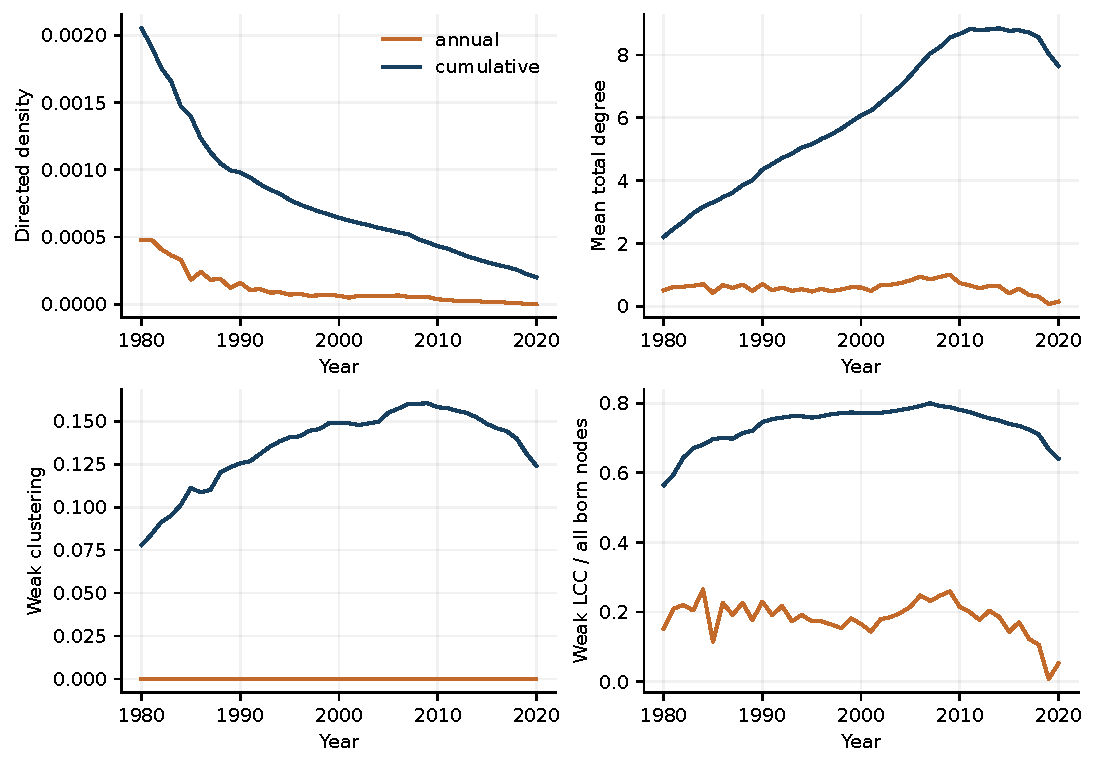
\includegraphics[width=.95\textwidth]{b_aggregation.pdf}
\caption{Measured CIT annual and cumulative structure, including born isolates.
The annual zero clustering is imposed by strict publication-year ordering.}
\label{fig:b-aggregation}
\end{figure*}

\paragraph{Window interpretation.}
\Cref{fig:b-window} shows that longer windows connect a larger fraction of born
papers and admit cross-year triangles. These effects require a sequence of
snapshots; one final aggregate cannot reveal when connectivity appears.
The relative range is a window-sensitivity statistic, not a significance test
against a temporal null, and identical density/degree sensitivity follows from
the common denominator.

\begin{figure*}[t]
\centering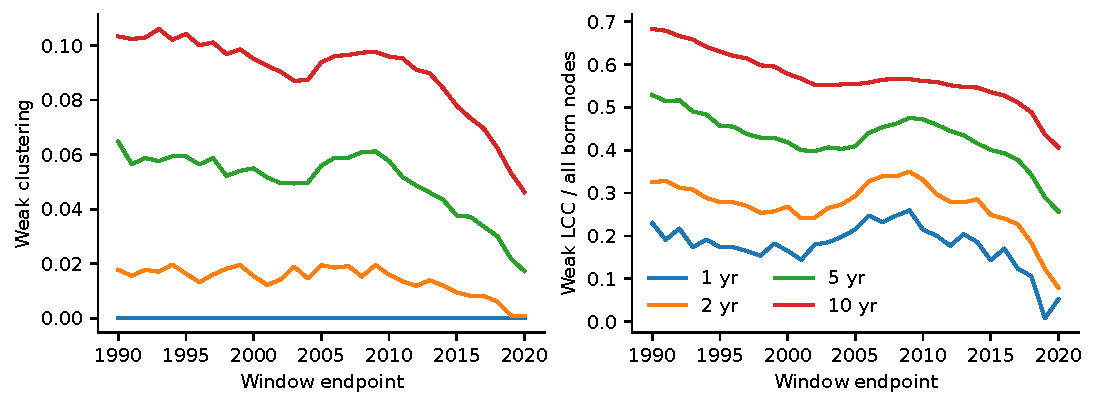
\includegraphics[width=.95\textwidth]{b_window_sensitivity.pdf}
\caption{Measured CIT trailing-window clustering and connectivity for 1, 2, 5
and 10 years. Born isolates are included at every endpoint.}
\label{fig:b-window}
\end{figure*}


\paragraph{Verdict on H1.}
Supported for CIT under the stated node denominator and strict-year convention.
A comparative verdict for PS and CM awaits their measurements; the relative
sensitivity of network types cannot yet be ranked.
 % Part I   (A, B)
\subsection{Activity patterns}
\label{sec:r-activity}

% Owner: C
\paragraph{Burstiness and memory.}
\expect{[Expected] Inter-event times of both PS and CM are heavy-tailed and have
positive burstiness $B$ and memory $M$. Under P1 the heavy tail is largely
removed, so $B_{\mathrm{real}}-B_{\mathrm{null}}>0$. Contact bursts in PS are
bounded by the school timetable, while CM shows longer waiting times (hours to
days) and a stronger tail.}

\begin{figure}[t]
\centering
\figph{\columnwidth}{3.6cm}{inter-event time distributions, real vs.\ P1\\(PS, CM)}
\caption{Inter-event time distributions on log--log axes. (Placeholder.)}
\label{fig:iet}
\end{figure}

\begin{table}[t]
\centering
\small
\begin{tabular}{@{}lcccc@{}}
\toprule
 & \multicolumn{2}{c}{PS} & \multicolumn{2}{c}{CM} \\
 & real & P1 & real & P1 \\
\midrule
Burstiness $B$ & $>0$ & $\approx$ lower & $>0$ & $\approx$ lower \\
Memory $M$ & $>0$ & $\approx 0$ & $>0$ & $\approx 0$ \\
\bottomrule
\end{tabular}
\caption{Expected qualitative outcome of M2a (values to be measured; mean $\pm$
std over $\geq 20$ P1 samples).}
\label{tab:burst}
\end{table}

% Owner: C
\paragraph{Persistence and turnover.}
\expect{[Expected] Many contacts in PS are repeated within the same day (within
class), so the edge repetition rate is high and consecutive-snapshot Jaccard is
moderate, with drops at class changes. In CM most pairs interact only a few
times, so tie lifetimes are short and turnover is high. P1 keeps the static graph
and therefore the repetition rate, but changes lifetimes and Jaccard.}

\paragraph{Verdict on H2 and H3.}
\outline{Supported / not supported / depends on network type or window.}
\expect{[Expected] H2 supported in both. H3 supported in PS, only partly in CM.}
    % Part II  (C)
\subsection{Structural evolution}
\label{sec:r-evolution}

% Owner: B
% Owner: B -- measured M2c-1 through M2c-4 only.
\paragraph{Preferential attachment (H4a).}
The conditional kernel $(k+1)^\alpha$ gives $\alpha=0.714$, with a descriptive
95\% year-bootstrap interval $[0.693,0.730]$. Twenty P3a samples yield
$0.0006\pm0.0051$ and age-only P3b yields $-0.6512\pm0.0053$.
The observed exponent exceeds all null values (empirical one-sided probability
$1/21$ per comparison, with coarse resolution). The exponent stays positive
under time splits, offsets 0.5/2 and a core venue-family subset.
\textbf{Verdict:} sublinear degree preference is supported within this corpus,
beyond the age-only reference; this does not identify a causal PA mechanism.

\paragraph{Ageing (H4b).}
Lognormal target preference is preferred to exponential, power-law and uniform
kernels, with respective $\Delta$AIC 537.8, 9,360.5 and 41,796.7.
The lognormal parameters are $(\mu,\sigma)=(1.858,1.108)$; its underlying scale
$e^\mu$ is 6.41 years. Mean age over all retained citations is 5.711 years, versus
$11.457\pm0.034$ for P3a and $5.717\pm0.018$ for calibrated P3b.
Lognormal is preferred in all three target cohorts, although recent-cohort tails
remain censored. \textbf{Verdict:} age-independent choice is inadequate;
P3b's agreement is calibration, not independent confirmation of ageing.

\begin{figure*}[t]
\centering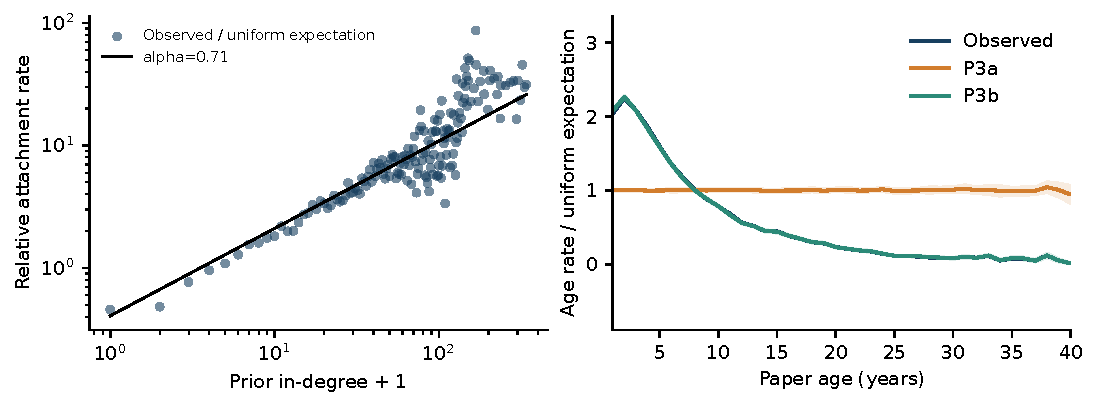
\includegraphics[width=.95\textwidth]{b_attachment_ageing.pdf}
\caption{Measured CIT attachment and exposure-adjusted age preference.
Points with at least five hits are displayed; the exponent uses all supported
classes with yearly normalization. Null bands show mean $\pm$ SD.}
\label{fig:growth}
\end{figure*}

\paragraph{Densification and diameter (H4c).}
For 1990--2020, $a=1.343$ ($R^2=0.991$), with descriptive year-resampling
interval $[1.288,1.406]$. Growth is weaker in 2005--2020 ($a=1.065$) than
1990--2004 (1.455); cutoff 2015 gives 1.427, inclusion of year ties 1.324,
and the core venue subset 1.410. Densification is superlinear edge growth,
not increasing directed density. The sampled weak-LCC effective diameter is
6 hops in every year; 64/256-source endpoint checks agree.
P3 fixes $N(t)$ and $E(t)$, hence also $a$.
\textbf{Verdict:} densification is observed, but diameter shrinkage is not
detected at the sampled 90th-percentile resolution.

\begin{figure*}[t]
\centering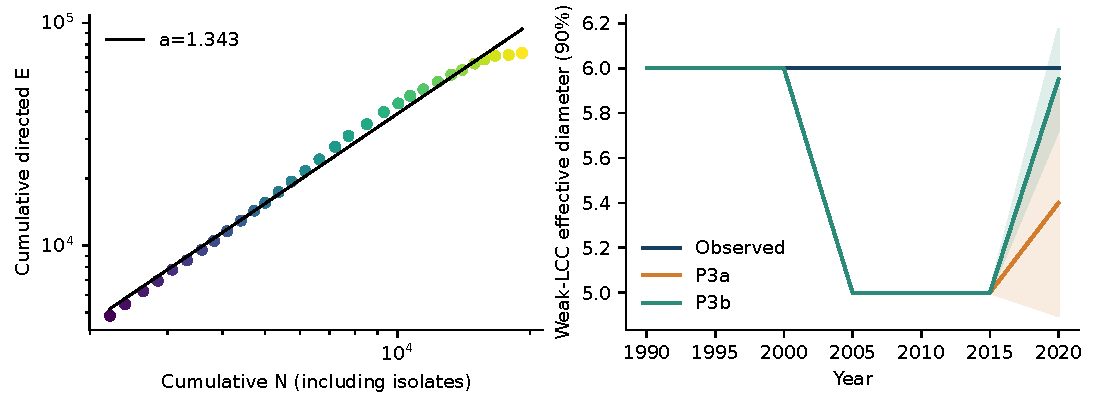
\includegraphics[width=.95\textwidth]{b_densification_diameter.pdf}
\caption{CIT cumulative growth and effective diameter. Null diameter means and
SD are estimated every five years. P3 cannot test densification significance
because its source reference counts are fixed.}
\label{fig:b-densification}
\end{figure*}

\paragraph{Citation dynamics and prediction (H4d).}
For 500 full-history fits, median WSB parameters are
$(\lambda,\mu,\sigma)=(2.717,0.834,1.238)$, median RMSLE is 0.074 and
scaled-collapse RMSE is 0.022. These are fitted-sample diagnostics.
On 500 papers selected using only their first five years, age-15 MAE is
15.144 for WSB, 17.064 for linear extrapolation and 27,588 for no-ageing PA;
at the observed 2020 endpoint it is 28.016, 27.271 and $2.79\times10^6$.
The paired MAE differences WSB minus linear have 95\% intervals
$[-4.471,0.806]$ and $[-4.764,8.128]$, both including zero. Forecast fits hit
parameter bounds for 38.6\% of papers; all remain in primary scoring.
\textbf{Verdict:} compact descriptive fits are supported, but a clear predictive
advantage over the simple linear baseline is not established. Observed-endpoint
citations are censored within-corpus counts, not lifetime impact.

\begin{figure*}[t]
\centering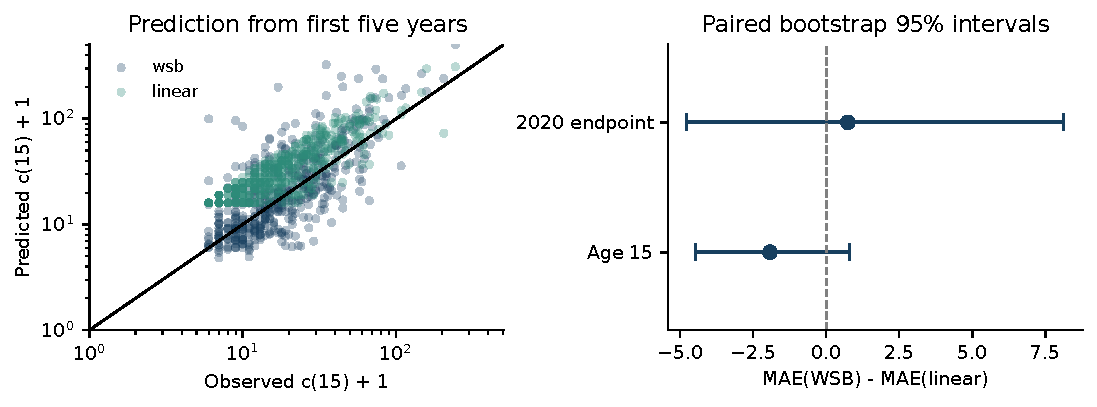
\includegraphics[width=.95\textwidth]{b_wsb_validation.pdf}
\caption{WSB held-out prediction and paired MAE differences versus linear.
Both bootstrap intervals cross zero; fitted collapse alone does not establish
long-term predictability.}
\label{fig:b-wsb-validation}
\end{figure*}


% Owner: E
\paragraph{Dynamic vs.\ static communities.}
\expect{[Expected] In PS the static partition recovers the classes well, but
snapshots reveal mixing during breaks and re-formation of classroom groups during
lessons, so consecutive NMI is moderate and fluctuates with the timetable. In CM
snapshot communities are unstable (low consecutive NMI), and P1 lowers
consecutive NMI further. Results should be insensitive to the resolution parameter
within a reasonable range.}

\begin{table}[t]
\centering
\small
\begin{tabular}{@{}lcc@{}}
\toprule
 & PS & CM \\
\midrule
Consecutive NMI & medium & low \\
Dynamic vs.\ static NMI & medium & low \\
NMI with classes & high (static) & -- \\
\bottomrule
\end{tabular}
\caption{Expected qualitative outcome of M4 (values and P1 baseline to be measured).}
\label{tab:nmi}
\end{table}

\paragraph{Verdict on H5.}
\outline{Supported / not supported / depends on network type or window.}
\expect{[Expected] H5 supported for CM, and in PS tied to
the daily timetable.}
   % Part III (B, E)
\subsection{Paths, centrality and spreading}
\label{sec:r-function}

% Owner: D
\paragraph{Reachability.}
\expect{[Expected] The fraction of pairs connected by a time-respecting path is
well below the static value in both networks. Under P1 reachability changes
because temporal order is destroyed, whereas P2 changes it through topology,
so the two nulls attribute the loss to different causes.}

\begin{figure}[t]
\centering
\figph{\columnwidth}{3.4cm}{reachability ratio $R$: real, P1, P2 (PS, CM)}
\caption{Temporal reachability ratio, real vs.\ P1 and P2. (Placeholder.)}
\label{fig:reach}
\end{figure}

% Owner: E
% Owner: E. M3b / H6 (rankings), input from results_function.tex.
% Values: results/e_summary.csv and results/e/m3b_*; figure: scripts/plot_e.py.
\begin{table}[t]
\centering
\small
\begin{tabular}{@{}llcc@{}}
\toprule
 & Measure & Real & P1 \\
\midrule
PS & $\tau$, unweighted & 0.71 & $0.55\pm0.01$ \\
   & $\tau$, weighted & 0.39 & $0.69\pm0.01$ \\
   & top-10\%, unweighted & 0.50 & $0.51\pm0.07$ \\
   & top-10\%, weighted & 0.29 & $0.60\pm0.06$ \\
\midrule
CM & $\tau$, unweighted & 0.78 & $0.85\pm0.00$ \\
   & $\tau$, weighted & 0.74 & $0.86\pm0.00$ \\
   & top-10\%, unweighted & 0.65 & $0.74\pm0.01$ \\
   & top-10\%, weighted & 0.57 & $0.72\pm0.02$ \\
\bottomrule
\end{tabular}
\caption{Agreement of static and temporal closeness rankings: Kendall $\tau_b$ and
overlap of the top 10\% nodes. P1: temporal closeness on 20 samples (mean $\pm$ sd); the
static ranking is unchanged by P1.}
\label{tab:m3b}
\end{table}

\begin{figure*}[t]
\centering
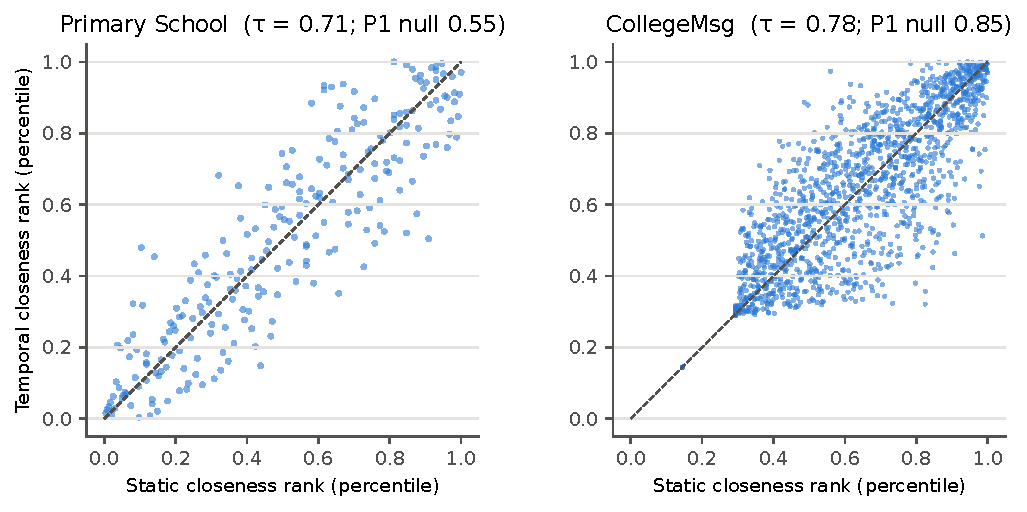
\includegraphics[width=0.8\linewidth]{e_m3b_rank_scatter.pdf}
\caption{Static (unweighted harmonic) vs.\ temporal closeness rank of every node; dashed:
identical rankings. The tied block at the lower left of the CM panel is the 29\% of users
who never send a message.}
\label{fig:m3b}
\end{figure*}

\paragraph{Centrality.}
Static and temporal closeness rankings are clearly correlated in both networks
(\cref{tab:m3b,fig:m3b}; $\tau=0.71$ in PS and $0.78$ in CM, hop distance), so the static
network shows roughly which nodes are central. It is much less reliable about which nodes
are \emph{most} central: only half of the PS top 10\% and two thirds of the CM top 10\%
coincide. In CM the real agreement is somewhat lower than under P1 (0.78 vs.\ 0.85), so
event order makes static closeness a slightly worse guide. The CM $\tau$ is also helped by
the 549 users (29\%) who never send a message and have zero closeness in both rankings
(the tied block in \cref{fig:m3b}).

In PS the effect depends on edge weights. Weighted static closeness agrees poorly with
temporal closeness ($\tau=0.39$, top-10\% overlap 0.29), whereas after P1 the agreement
is high ($0.69\pm0.01$). In the school, most contact weight comes from repeated contacts
within a class during lessons; these happen while the class is already connected and
hardly shorten time-respecting paths to the rest of the school. Under P1 the same contacts
are spread over the day, and a heavy edge becomes a frequent chance to transmit. Without
weights the effect reverses (real 0.71 vs.\ P1 0.55): reaching the school quickly depends
on having many distinct partners, which in PS largely means mixing at breaks.

\emph{Rankings part of H6: partly supported.} The rankings are correlated
($\tau=0.71$--$0.78$) but the top nodes differ by 35--50\%, and in face-to-face data
weighting edges by contact frequency makes the static ranking misleading ($\tau=0.39$).


% Owner: D
\paragraph{Spreading.}
\expect{[Expected] SIR epidemics on the real sequences peak later than on P1,
$T_{\mathrm{real}}/T_{\mathrm{null}}>1$, and the effect is larger for the
burstier CM. In PS, the final size is limited by the timetable (outbreaks pause
overnight).}

\begin{figure}[t]
\centering
\figph{\columnwidth}{3.4cm}{SIR prevalence curves: real, P1, P2 (PS, CM)}
\caption{Mean SIR prevalence with $\geq 100$ seeds. (Placeholder.)}
\label{fig:sir}
\end{figure}

\paragraph{Verdict on H6 and H7.}
\outline{Supported / not supported / depends on network type or window.}
\expect{[Expected] H6 supported in both networks. H7 supported, strongest for CM.}
    % Part IV  (D, E)
\subsection{CIT model diagnostics and robustness}
\label{sec:b-diagnostics}
% Owner: B. All diagnostics use the completed CIT run, not new experiments.
\paragraph{Null controls and ageing alternatives.}
\Cref{fig:b-null-age} visualizes the separation of the observed attachment
exponent from both null ensembles and the age-kernel AIC comparison.
P3b matches mean citation age because its age weights were fitted to these data;
that agreement is a property of the control, not independent evidence for ageing.
With only 20 realizations per null, an observed value above all nulls has empirical
one-sided probability $1/21$; this does not justify a precise tail estimate.
The ageing comparison is on identical risk sets and observations.

\begin{table}[t]
\centering\small
\begin{tabular}{@{}lrr@{}}
\toprule
Age kernel & Parameters & $\Delta$AIC\\
\midrule
Lognormal & 2 & 0.0\\
Exponential & 1 & 537.8\\
Power-law & 1 & 9,360.5\\
Uniform & 0 & 41,796.7\\
\bottomrule
\end{tabular}
\caption{CIT age-preference alternatives on common observed support. AIC selects
among the declared models, not among every possible ageing mechanism.}
\label{tab:b-age-models}
\end{table}

\begin{figure*}[t]
\centering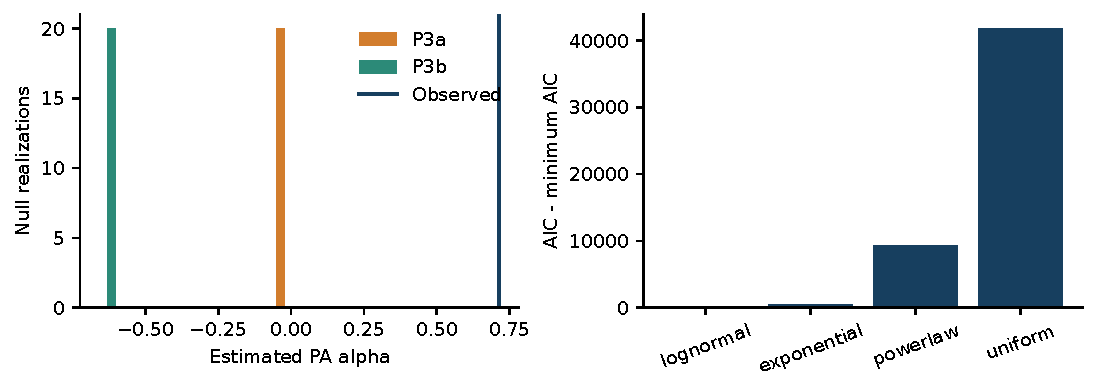
\includegraphics[width=.95\textwidth]{b_null_and_age_models.pdf}
\caption{CIT null-model attachment exponents and age-kernel AIC differences.
Uniform P3a and calibrated age-only P3b each have 20 independent realizations.}
\label{fig:b-null-age}
\end{figure*}

\paragraph{Fit quality does not establish predictability.}
The full-history sample is 500 of 1,019 papers with at least ten citations by age
15; the forecast sample is 500 of 1,220 eligible papers selected only by having
at least five citations in their first five years. Both samples are drawn with a
fixed seed. Median full-history RMSLE is 0.0736 and median scaled-collapse RMSE
0.0220 (90th percentile 0.0453); 10.2\% of full-history fits hit a parameter bound.
\Cref{fig:b-wsb-fits} is an in-sample diagnostic. Held-out scoring in
\cref{tab:b-forecast} and \cref{fig:b-wsb-validation} provides the separate
predictive test. In particular, a collapse obtained using parameters fitted to
the same curve is not independent evidence for universal citation dynamics.

\begin{figure*}[t]
\centering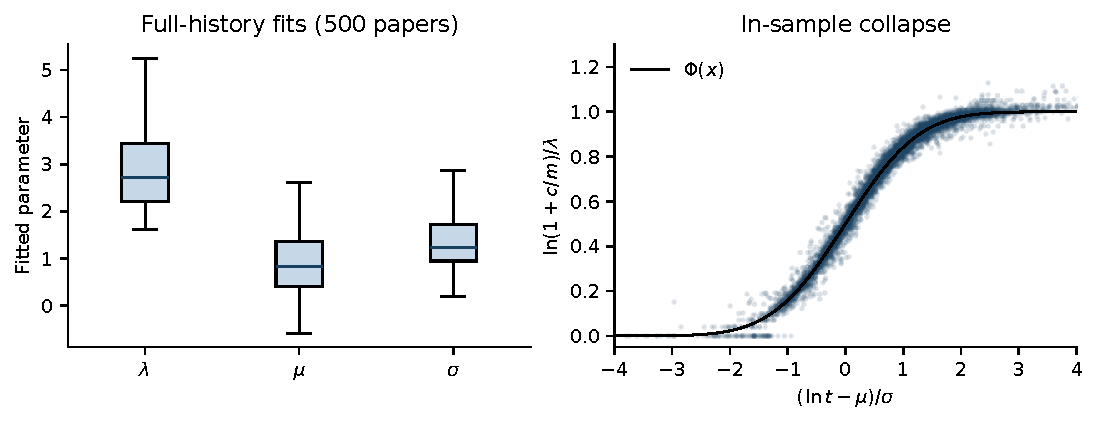
\includegraphics[width=.95\textwidth]{b_wsb_fit_diagnostics.pdf}
\caption{WSB full-history diagnostics: parameter distributions (boxes are
interquartile ranges, median lines, standard 1.5-IQR whiskers; outliers hidden)
and the scaled citation histories against $\Phi(x)$. Parameters are fitted to
ages 1--15, so the collapse is descriptive, not held-out validation.}
\label{fig:b-wsb-fits}
\end{figure*}

\begin{table}[t]
\centering\small
\setlength{\tabcolsep}{4pt}
\begin{tabular}{@{}llrr@{}}
\toprule
Target & Model & MAE & RMSLE\\
\midrule
15 yr & WSB & 15.144 & 0.601\\
 & Linear & 17.064 & 0.662\\
 & No-age PA & 27,588 & 4.601\\
\midrule
2020 & WSB & 28.016 & 0.778\\
 & Linear & 27.271 & 0.876\\
 & No-age PA & $2.79\!\times\!10^6$ & 7.000\\
\bottomrule
\end{tabular}
\caption{Matched forecasts on 500 selected papers using only years 1--5 for
training. The 2020 target is the observed, censored corpus endpoint.
The exponential no-age PA baseline over-extrapolates; beating it alone is a weak
test. The paired MAE intervals against linear both include zero.}
\label{tab:b-forecast}
\end{table}

\paragraph{Sensitivity of the conclusions.}
\Cref{tab:b-robustness} reports time splits, cutoff and corpus-selection checks.
The sign of degree preference and superlinear full-period growth persist, but
$a$ is substantially weaker in the late period. Degree offsets 0.5 and 2 give
$\alpha=0.604$ and 0.858, so the numerical exponent is convention-dependent.
Including 5,486 year ties gives $a=1.324$; ties remain excluded from the primary
DAG. Effective-diameter endpoint estimates remain 6 hops with 64, 128 or 256
sources. First-ten versus all-twenty null means of $\alpha$ are 0.00055/0.00059
(P3a) and $-0.65320$/$-0.65118$ (P3b).
Lognormal ageing is preferred in all target cohorts and both observation halves,
but the recent cohort's fitted tail extends beyond its observed follow-up.
These checks support qualitative stability without eliminating coverage bias,
right censoring or unobserved fitness.

\begin{table}[t]
\centering\small
\begin{tabular}{@{}lrr@{}}
\toprule
Variant & $\alpha$ & $a$\\
\midrule
1990--2020 (primary) & 0.714 & 1.343\\
1990--2004 & 0.684 & 1.455\\
2005--2020 & 0.721 & 1.065\\
Cutoff 2015 & 0.722 & 1.427\\
Core venue families & 0.731 & 1.410\\
Same-year edges included & -- & 1.324\\
\bottomrule
\end{tabular}
\caption{CIT robustness from the saved run. Core venue families contain 14,235
nodes and 47,009 primary edges; the year-tie variant is structural only.}
\label{tab:b-robustness}
\end{table}

\subsection{Measured hypothesis summary}
\label{sec:r-cross}
% Owner: A for eventual cross-network synthesis; B supplies the measured CIT cells.
\Cref{tab:cross} separates available CIT evidence from pending PS/CM experiments.
No ordering of network types by temporal sensitivity is established until the
same normalized measures have been computed for all applicable datasets.
The split H4 verdict avoids treating densification, diameter shrinkage,
descriptive fit and predictive superiority as one interchangeable claim.

\begin{table}[t]
\centering\small
\setlength{\tabcolsep}{4pt}
\begin{tabular}{@{}lcc p{3.8cm}@{}}
\toprule
ID & PS & CM & Measured CIT evidence \\
\midrule
H1 & Pending & Pending & Relative ranges: density/degree 1.798, clustering 2.361, LCC 1.114.\\
H2 & Pending & Pending & --\\
H3 & Pending & Pending & --\\
H4a & -- & -- & $\alpha=0.714$ [0.693, 0.730]; sublinear degree preference.\\
H4b & -- & -- & Lognormal preferred; scale 6.41 yr; $\Delta$AIC versus exponential 537.8.\\
H4c & -- & -- & $a=1.343$; $D_{90}=6$ throughout. Densification, no detected shrinkage.\\
H4d & -- & -- & Compact fits; MAE advantage over linear unresolved.\\
H5 & Pending & Pending & --\\
H6 & Pending & Pending & --\\
H7 & Pending & Pending & --\\
\bottomrule
\end{tabular}
\caption{Available evidence. Pending denotes unmeasured PS and CM experiments;
-- denotes inapplicability. CIT intervals are descriptive year resamples.
H4c/H4d have mixed verdicts. Values come from the shared summary and supporting tables.}
\label{tab:cross}
\end{table}
       % summary  (A assembles)

\FloatBarrier

%=====================================================================
\section{Discussion}
\label{sec:discussion}

\paragraph{What the static network already tells us.}
Conclusions that survive aggregation can be read from \cref{tab:cross}.
For CIT, the final aggregate describes degree heterogeneity, clustering and
connected components. It cannot by itself identify preferential attachment or
ageing: these compare new citations with prior degrees and paper ages.
Even densification requires a sequence of historical $N(t),E(t)$ pairs, rather
than one final graph. The PS/CM claims remain to be tested.

\paragraph{What requires time.}
Some conclusions need windows (Parts I and III) and others the full event order
(Parts II and IV).
\expect{[Expected] Burstiness, turnover, community reorganisation, time-respecting
reachability and spreading speed cannot be obtained from the aggregate.}

\paragraph{Why network types differ.}
The three networks differ in generating mechanism (physical proximity, voluntary
messaging, citing earlier work), time scale and edge semantics (a contact ends, a
message is a point event, a citation persists).
\expect{[Expected] Proximity is constrained by timetables and space and thus has
strong periodic structure, messages are driven by individual bursty decisions.}
CIT has persistent edges and measured age-dependent target preferences.
A cross-network ordering still needs PS/CM measurements.

\paragraph{Robustness.}
We check the choice of window size, the observation period (first vs.\ second
half), the community-detection resolution and the choice of null model.
For CIT, the full-period densification exponent is 1.343 but falls to 1.065 in
the later half, while remaining 1.427 with cutoff 2015. Positive degree preference
persists under all declared variants, although its exponent depends on the degree
offset. The diameter verdict is unchanged by the sampled-source sensitivity
checks. These are qualitative robustness findings, not evidence that coverage
and censoring have been removed.


% Owner: B (measured citation-specific interpretation).
\paragraph{Citation-specific evidence.}
CIT supports degree preference and age-dependent target choice, but separates two
claims often grouped together: cumulative edges grow superlinearly, while the
sampled effective diameter does not shrink. A three-parameter citation curve
fits selected histories well, yet its paired MAE advantage over linear prediction
is unresolved. Annual zero clustering is imposed by the strict-year snapshot
construction. These examples show why representation, fitted-sample description
and held-out prediction require separate interpretations. Late reference coverage,
within-venue selection and right censoring constrain all citation conclusions.

\paragraph{Limitations.}
There is one dataset per network type, so generality is limited and conclusions
hold ``in these data''. CIT also has within-venue sampling, annual timestamp ties and changing reference
coverage. Its year-block bootstrap intervals are descriptive; cumulative graph
observations are dependent. The 20-draw null ensembles give coarse tail resolution.
Forecast selection excludes low-cited papers, and 38.6\% of short-history WSB fits
hit parameter bounds; fitted collapse is not independent validation.
Boundary effects
and sampling bias remain (finite two-day contact window, sensor participation).
Citation networks are degenerate temporal networks (DAG, no deletion), which is
why several methods do not apply. Each system also contains several time scales
\citep{holme2015modern}, so a window that suits one process may hide another. Finally, SocioPatterns data are released under
CC BY-NC-SA.

%=====================================================================
\section{Conclusion}
\label{sec:conclusion}
The completed citation-network experiments show that the importance of time
depends on the question. A final aggregate reveals degree heterogeneity and
connectivity, while preferential attachment, ageing and the growth law require
historical degrees, publication ages or cumulative snapshots. In the selected
AMiner database corpus, sublinear degree preference and age-dependent citation
choice coexist with superlinear edge growth, yet the sampled effective diameter
does not shrink. WSB compactly describes selected citation histories, but its
mean-absolute-error advantage over a simple linear forecast is not established.
Thus descriptive fit, temporal mechanism and predictive value should be assessed
separately. PS/CM experiments remain pending, so conclusions about their dynamics
and a cross-network ranking of temporal sensitivity await measured evidence.
Future work includes broader corpus coverage, more datasets per type,
finer-resolution citation dates and predictive tests under alternative censoring
and missing-reference assumptions.


{\small
\bibliographystyle{ieeenat_fullname}
\bibliography{references}
}

\end{document}
